\chapter{Introdução}\label{cap:introducao}

Este relatório tem como objetivo principal apresentar uma análise numérica dos fenômenos de transferência de calor em aletas. Estas superfícies são consideradas como uma extensão de uma base condutora, potencializando o efeito da dissipação de calor.

O estudo se concentra em aletas planas unidimensionais e tem como objetivo determinar os principais fatores que influenciam a transferência de calor nesses tipos de superfícies. A análise será feita por meio de simulações numéricas que permitirão quantificar a transferência de calor e avaliar a eficiência das aletas em dissipar o calor de forma adequada.

Dentro do escopo do objetivo principal, foram definidos alguns objetivos específicos:

\begin{itemize}
   \item Determinar a temperatura da superfície da base da aleta (Tb);
   
   \item Determinar a taxa de transferência de calor de cada tipo de aleta (qa);
   
   \item Determinar a temperatura na ponta da aleta;
   
   \item Determinar a efetividade ({\large \(\epsilon\)}) da superfície estendida. Caso a aleta apresente ({\large\(\epsilon\)}1>2);

   \item Determinar a eficiência da aleta ({\large\(\eta\)}a);
   
   \item Determinar a eficiência global do conjunto aletado ({\large\({\eta}\)}o).
\end{itemize}

Para os cálculos, algumas grandezas foram fornecidas para facilitar na realização do trabalho.

\begin{table}[htb]
   \ABNTEXfontereduzida
   \centering
   \caption{Grandezas fornecidas}
   \label{tab:grandezasFornecidas}
   \begin{tabular}{p{8.15cm} r R{2.3cm}}\toprule
      Descrição & Grandeza & Valor\\
      \midrule
      Temperatura da superfície & \(T1\) & \SI{110}\degreeCelsius \\
      Temperatura do fluido ambiente em torno do conjunto & \(T\infty\) & \SI{30}\degreeCelsius \\
      Coeficiente de transferência de calor por convecção & \(h\) & \SI{20}{\watt\per\square\meter\per\kelvin} \\
      \bottomrule
   \end{tabular}
   \fonteproprioautor
\end{table}

apresentadas
 
\begin{figure}[ht]
	\centering
	\caption{Tabela propriedades termofísicas de sólidos metálicos selecionados}\label{fig:metalProps}
	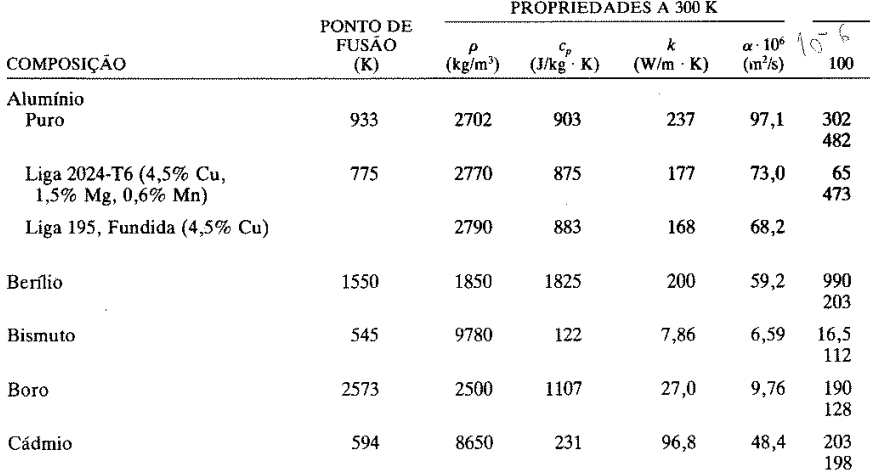
\includegraphics[width=15cm]{figuras/metalProps.jpg}
    \fonte{\citeonline{uspTabelasTermodinamicas}}
\end{figure}


\section{Objetivos}

Neste item deverá ser indicado claramente o que se deseja fazer, o que se pretende alcançar. É fundamental que estes objetivos sejam possíveis de serem atingidos. Geralmente se formula um objetivo geral articulando-o a outros objetivos mais específicos.

\subsection{Objetivo geral}

Procura-se determinar\footnote{Atenção! Inicie a frase com um verbo abrangente e no infinitivo, como: compreender, saber, avaliar, verificar, constatar, analisar, desenvolver, conhecer, entender, levantar, mapear, identificar.}, com clareza e objetividade, o seu propósito com a realização da pesquisa. Deve-se estar atento ao fato de que nesta pesquisa, em nível de graduação ou pós-graduação, os propósitos são essencialmente acadêmicos, como mapear, identificar, levantar, diagnosticar, traçar o perfil ou historiar determinado assunto específico dentro de um tema. Um objetivo bem redigido explica o quê, com o quê (quem), por meio de quê, onde, quando sobre a pesquisa.

\subsection{Objetivos específicos}

Significa aprofundar as intenções expressas no objetivo geral. Propõe-se mapear, identificar, levantar, diagnosticar, traçar o perfil ou historiar determinado assunto específico dentro de um tema. Assim, para elaborar os objetivos específicos deve-se:

\begin{itemize}
   \item detalhar o objetivo geral mostrando o que se pretende alcançar com a pesquisa;
   \item tornar operacional o objetivo geral, indicando exatamente o que será realizado na pesquisa;
   \item usar verbos que admitam poucas interpretações e no infinitivo, como: identificar, caracterizar, comparar, testar, aplicar, observar, medir, localizar, selecionar, distinguir.
\end{itemize}


\section{Organização do texto}

O texto está organizado da seguinte forma: No \autoref{cap:revisao} é apresentado um pouco mais de como fazer um outro capítulo, apresentando ainda formas para inserir figuras. No \autoref{cap:proposta} é apresentado uma forma para adicionar uma tabela. Por fim, no \autoref{cap:conclusoes} são apresentadas as conclusões sobre este trabalho.